% Article type supporting font formatting
\documentclass[a4,12pt]{extarticle}

% Define .tex file encoding
\usepackage[utf8]{inputenc}

% Norwegian language support
%\usepackage[norsk]{babel}     

% Indent first paragraph in section
\usepackage{indentfirst}

% Allows mathbb in tex file
\usepackage{amsfonts}    
     
% Margin defining package
\usepackage{geometry}         
\geometry{a4paper
  ,margin=1in
}

\usepackage[square,numbers]{natbib}

% For use of graphics in document
\usepackage{graphicx}         

% Allows multi-line comments in tex file
\usepackage{verbatim}         

% Allows math in tex file 
\usepackage{amsmath}          

% Allows math symbols in tex file
\usepackage{amssymb}          

% Allows use of physics shortcut functions
%\usepackage{physics}          

% Verbatim env with LaTeX commands
\usepackage{alltt}            

% Allows \begin{figure}[H]
\usepackage{float}            

% Necessary for defining colours
\usepackage{color}            
\definecolor{linkgreen}{rgb}{0,.5,0}
\definecolor{linkblue}{rgb}{0,0,.5}
\definecolor{linkred}{rgb}{.5,0,0}
\definecolor{blue}{rgb}{.13,.13,1}
\definecolor{green}{rgb}{0,.5,0}
\definecolor{red}{rgb}{.9,0,0}

% Hyperlinks in document
\usepackage{hyperref}  
\hypersetup{
  colorlinks=true,     % True for colored links
  linktoc=all,         % True for table of contents links
  linkcolor=linkblue,  % Colour for links
  urlcolor=linkgreen,  % Colour for URLs
  citecolor=linkred    % Colour for citations
}

% Listing package for code examples
\usepackage{listings}         
\lstset{
  language=C++,                % Set language to C++
  showspaces=false,            % Don't show space chars
  showtabs=false,              % Don't show tab chars
  breaklines=true,             % Break long lines of code
  showstringspaces=false,      % Don't show spaces in strings
  breakatwhitespace=true,      % Break at white space only
  commentstyle=\color{green},  % Set colour for comments
  keywordstyle=\color{blue},   % Set colours for keywords
  stringstyle=\color{red},     % Set colour for strings
  basicstyle=\ttfamily,        % Set basic style
  tabsize=2                    % Set tabsize
}

% Referencing, last for compatibility reasons
\usepackage[noabbrev]{cleveref}

% Command to set two lines under text
\newcommand{\uunderline}[1]{\underline{\underline{#1}}}

% Command to use integral with limits
\newcommand{\Int}{\int\limits}    

% Command to use double integral with limits
\newcommand{\IInt}{\iint\limits}  

% Command to use triple integral with limits
\newcommand{\IIInt}{\iiint\limits}

% Command removes section numbering
\newcommand{\mysection}[2]{   
\setcounter{section}{#1}
\section*{#2}
\addcontentsline{toc}{section}{#2}
}

% Command removes subsection numbering
\newcommand{\mysubsection}[2]{  
\setcounter{subsection}{#1}
\subsection*{#2}
\addcontentsline{toc}{subsection}{#2}
}

% Command removes subsubsection numbering
\newcommand{\mysubsubsection}[2]{ 
\setcounter{subsubsection}{#1}
\subsubsection*{#2}
\addcontentsline{toc}{subsubsection}{#2}
}

% Makes matrices look square-ish
\renewcommand*{\arraystretch}{1.5}

%%%%%%%%%%%%%%%%%%%%%%%%%%%%%%%%%%%%%%%
%%      Title, Author, and Date      %%
%%%%%%%%%%%%%%%%%%%%%%%%%%%%%%%%%%%%%%%
\title{Assignment 4 in Artificial Intelligence\\Spring 2018 }
\author{Daniel Aaron Salwerowicz}
\date{\today}

%%%%%%%%%%%%%%%%%%%%%%%%%%%%%%%%%%%%%%%
%%           Start document          %%
%%%%%%%%%%%%%%%%%%%%%%%%%%%%%%%%%%%%%%%
\begin{document}
  
%%%%%%%%%%%%%%%%%%%%%%%%%%%%%%%%%%%%%%%
%%   Create the main title section   %%
%%%%%%%%%%%%%%%%%%%%%%%%%%%%%%%%%%%%%%%
\maketitle

%%%%%%%%%%%%%%%%%%%%%%%%%%%%%%%%%%%%%%
%%  The main content of the report  %%
%%%%%%%%%%%%%%%%%%%%%%%%%%%%%%%%%%%%%%

\mysection{1}{Task 1}
\mysubsection{1}{a}
Initial R and Q matrices are as follows:
\begin{align*}
R =	
\begin{bmatrix}
0 &     0 & -\inf &     0 & -\inf & -\inf \\
0 &     0 &   -10 & -\inf &     0 & -\inf \\
-\inf &     0 &   -10 & -\inf & -\inf &   100 \\
0 & -\inf & -\inf &     0 &     0 & -\inf \\
-\inf &     0 & -\inf &     0 &     0 &   100 \\
-\inf & -\inf &   -10 & -\inf &     0 &   100 
\end{bmatrix} &
Q =	
\begin{bmatrix}
0 &   0 &   0 &   0 &   0 &   0 \\
0 &   0 &   0 &   0 &   0 &   0 \\
0 &   0 &   0 &   0 &   0 &   0 \\
0 &   0 &   0 &   0 &   0 &   0 \\
0 &   0 &   0 &   0 &   0 &   0 \\
0 &   0 &   0 &   0 &   0 &   0  
\end{bmatrix}
\end{align*}
They are initialized like that since Q-matrix is always set to zero at the start and R-matrix represents enviromental values. As I have interpreted it there's no penalty for staying in the same room or for moving between rooms that were not specified in text. Therefore only moves that end up in room 3 or 6 have values other than zero associated with them. $-\inf$ is used to show that there is no connection between rooms ensuring that algorithm will never pick them.

Formula for calculating values in Q-matrix given learning factor $\alpha$ is 1:
\begin{align*}
Q(State,Action)=R(State,Action)+\gamma\cdot\text{Max}[Q(\text{Next S},\text{All A})]
\end{align*}

\mysubsection{2}{b}
\begin{align*}
Q(4,5)&=R(4,5)+\gamma\cdot\text{Max}[Q(5,1),Q(5,4),Q(5,5),Q(5,6)]\\
      &=0+0.9\cdot\text{Max}[0,0,0,0]\\
      &=0+0.9\cdot 0\\
Q(4,5)&=\uunderline{0}
\end{align*}

\mysubsection{3}{c}
\begin{align*}
Q(5,6)&=R(5,6)+\gamma\cdot\text{Max}[Q(6,3),Q(6,5),Q(6,6)]\\
      &=100+0.9\cdot\text{Max}[0,0,0]\\
      &=100+0.9\cdot 0\\
Q(5,6)&=\uunderline{100}
\end{align*}

\mysubsection{4}{d}
\begin{align*}
Q(4,5)&=R(4,5)+\gamma\cdot\text{Max}[Q(5,1),Q(5,4),Q(5,5),Q(5,6)]\\
      &=0+0.9\cdot\text{Max}[0,0,0,100]\\
      &=0+0.9\cdot 100\\
Q(4,5)&=\uunderline{90}
\end{align*}

\mysubsection{5}{e}
\begin{align*}
Q(1,4)&=R(1,4)+\gamma\cdot\text{Max}[Q(4,1),Q(4,4),Q(4,5)]\\
      &=0+0.9\cdot\text{Max}[0,0,90]\\
      &=0+0.9\cdot 90\\
Q(1,4)&=\uunderline{81}
\end{align*}

\mysubsection{6}{f}
Q matrix will look like this after going through all of the steps in b-e.
\begin{align*}
Q =	
\begin{bmatrix}
  0 &   0 &   0 &  81 &   0 &   0 \\
  0 &   0 &   0 &   0 &   0 &   0 \\
  0 &   0 &   0 &   0 &   0 &   0 \\
  0 &   0 &   0 &   0 &  90 &   0 \\
  0 &   0 &   0 &   0 &   0 & 100 \\
  0 &   0 &   0 &   0 &   0 &   0  
\end{bmatrix}
\end{align*}
Using this we can clearly see that the robot would take following path to the docking station:
$$1 \longrightarrow 4 \longrightarrow 5 \longrightarrow 6$$
Since:
$$Q(1,4)+Q(4,5)+Q(5,6)=81+90+100=171$$
Which is the highest possible reward using values defined in Q matrix.

\mysection{2}{Task 3}
\mysubsection{1}{a}
Going by the algorithm I will choose the splits so that S will be reduced as much as possible while keeping clean splits. Since I can have maximum of 4 regions I will only make three splits.

First split is going to be $x > 3$, since there are 4 red values in region defined by $x \leq 3$ and no blue values. So $(4,0)$.

Second split will be $y > 2$, since there are 3 red values in region defined by $y \leq 2$ and no blue values. So $(2,0)$.

Third and last split will be $y > 5.5$, since there are 5 blue values in region $y \leq 5.5$ and no red values. So $(0,5)$.

The remaining region will be majorly blue with 4 blue and 2 red values. So $(2,4)$.

Those splits are pretty much justified by the algorithm itself, since I tried to follow it as well as I could and understood it.

Resulting tree and regions can be found in \cref{Regions,Tree}.

\begin{figure}[H]
  \centering
  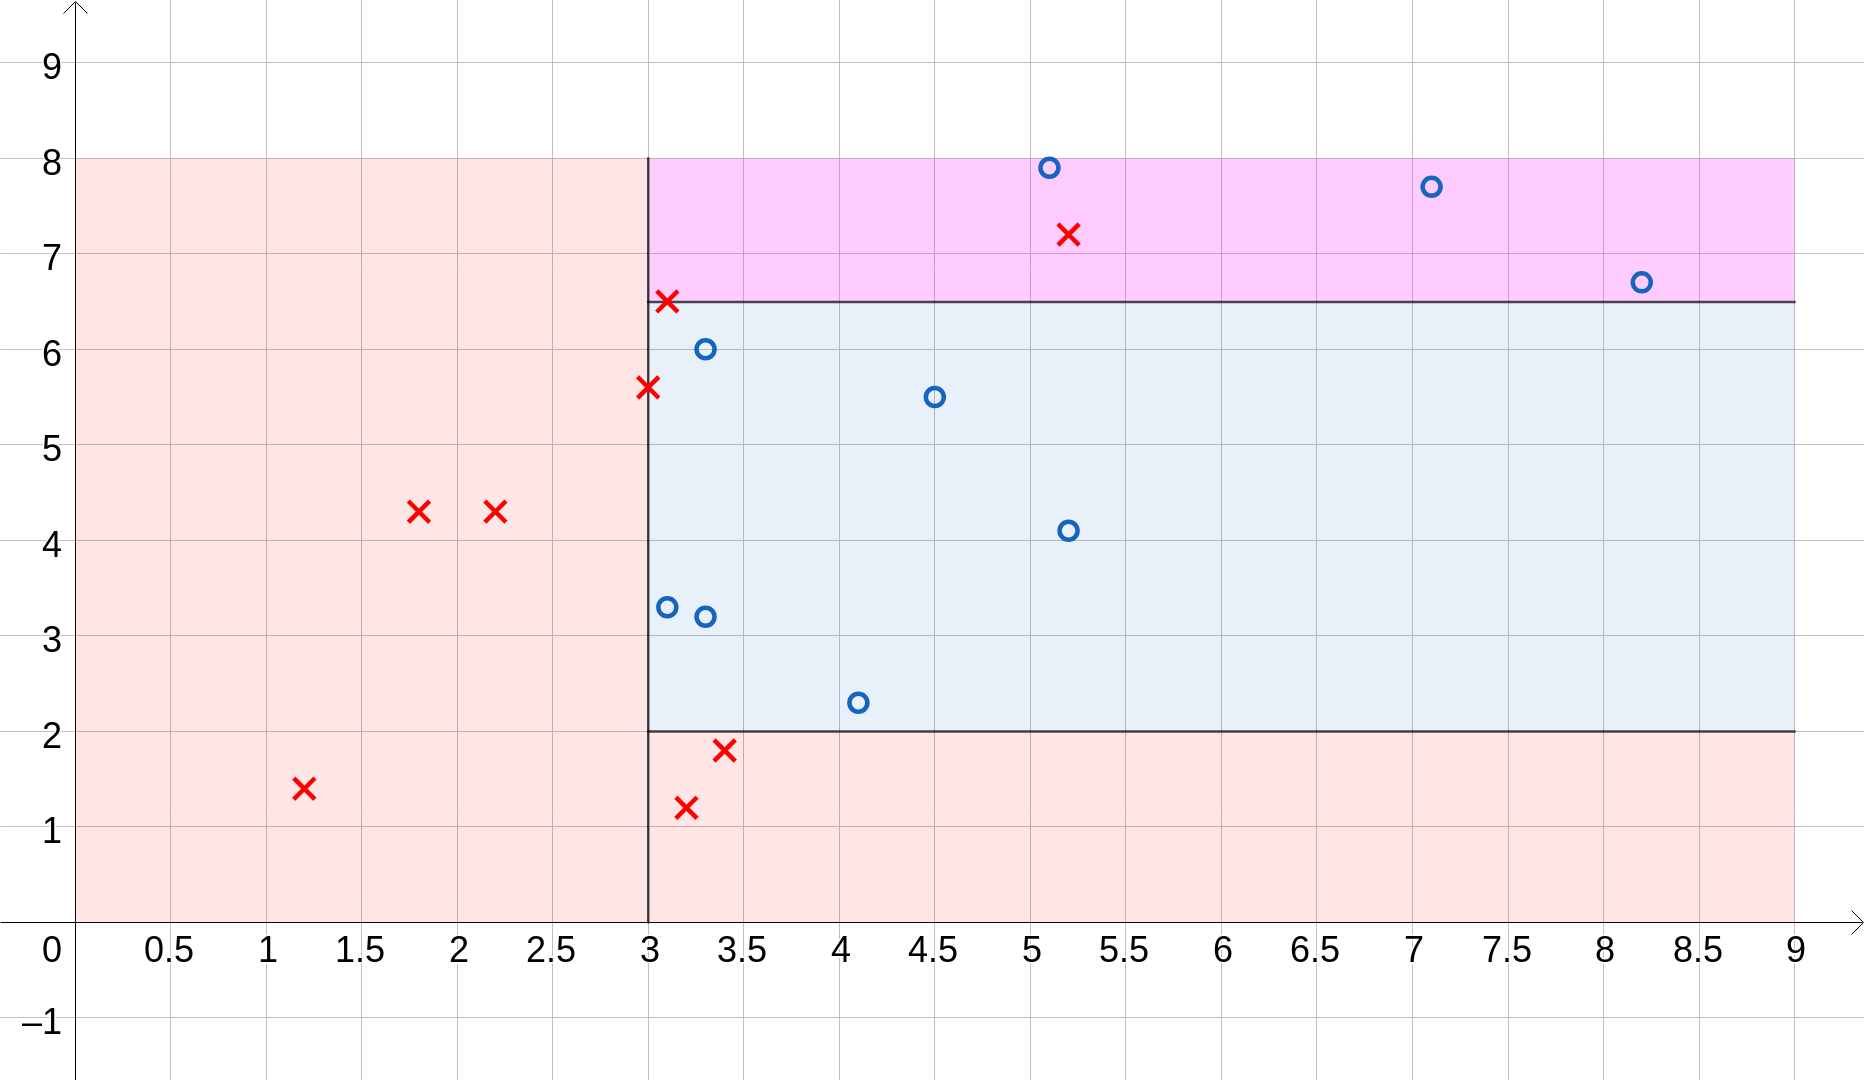
\includegraphics[width=.75\textwidth]{Regions}
  \caption{Regions split using the CART algorithm}
  \label{Regions}
\end{figure}
\begin{figure}[H]
\centering
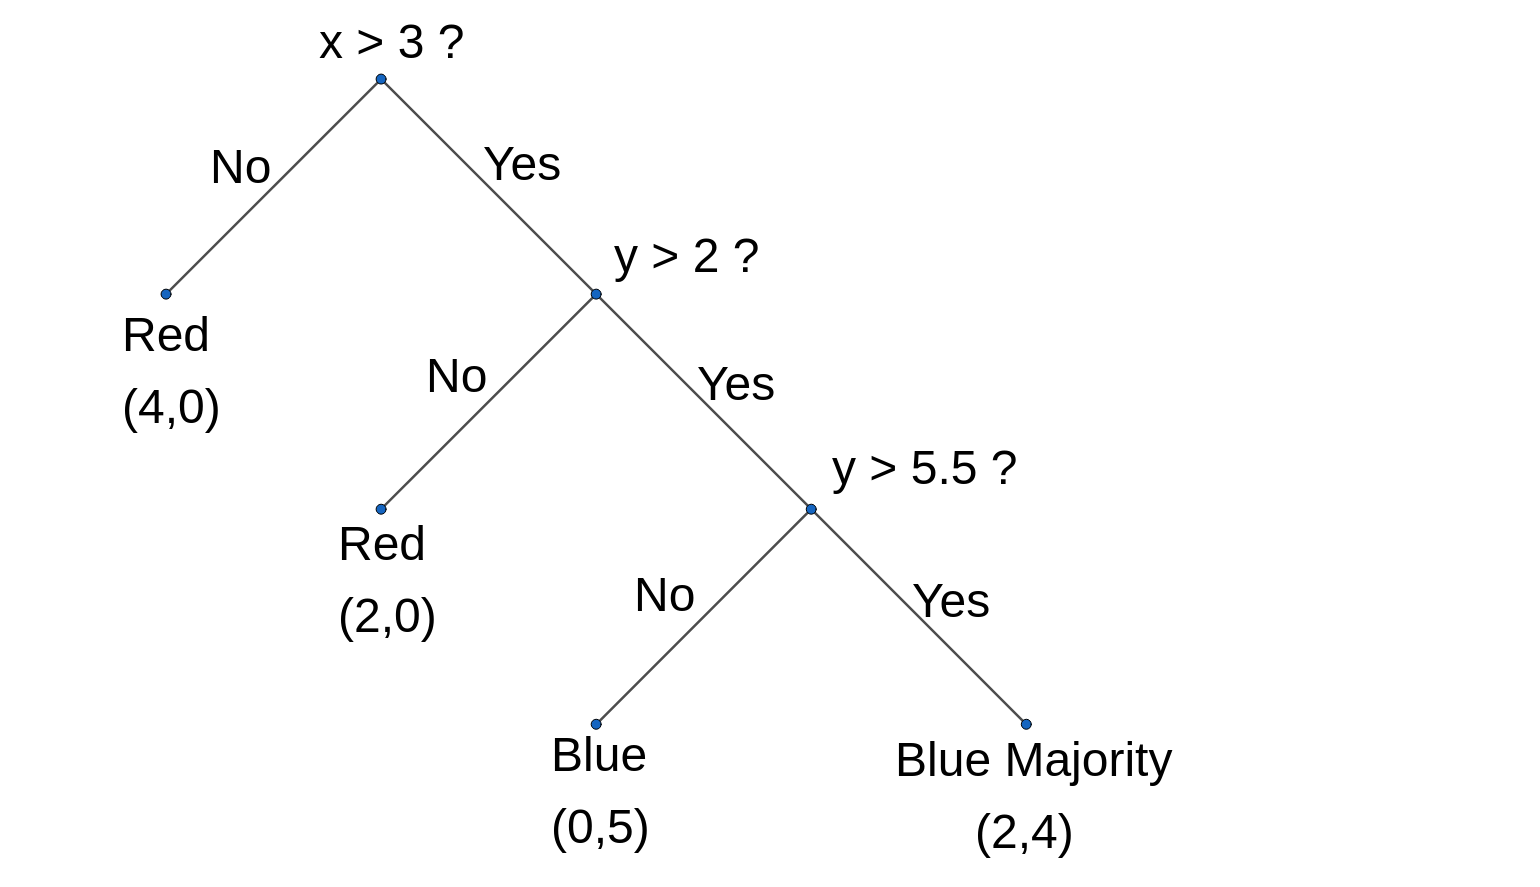
\includegraphics[width=.75\textwidth]{Tree}
\caption{Regression tree for the region above}
\label{Tree}
\end{figure}

\mysubsection{2}{b}
Plotting the test values $( 6.5 , 5.5 )$ and $( 4.1 , 6.5 )$ we can clearly see that the first point lands in the blue region, and is therefore defined as blue, whereas the second point falls in majorly blue region therefore there is $66.\overline{6}\%$ bias that it will be defined as blue and $33.\overline{3}\%$ bias that it will be defined as red. Therefore in my opinion and if my work is correct both of these points will be defined as blue. \Cref{NewValues} shows those new points plotted in the graph.

\begin{figure}[H]
  \centering
  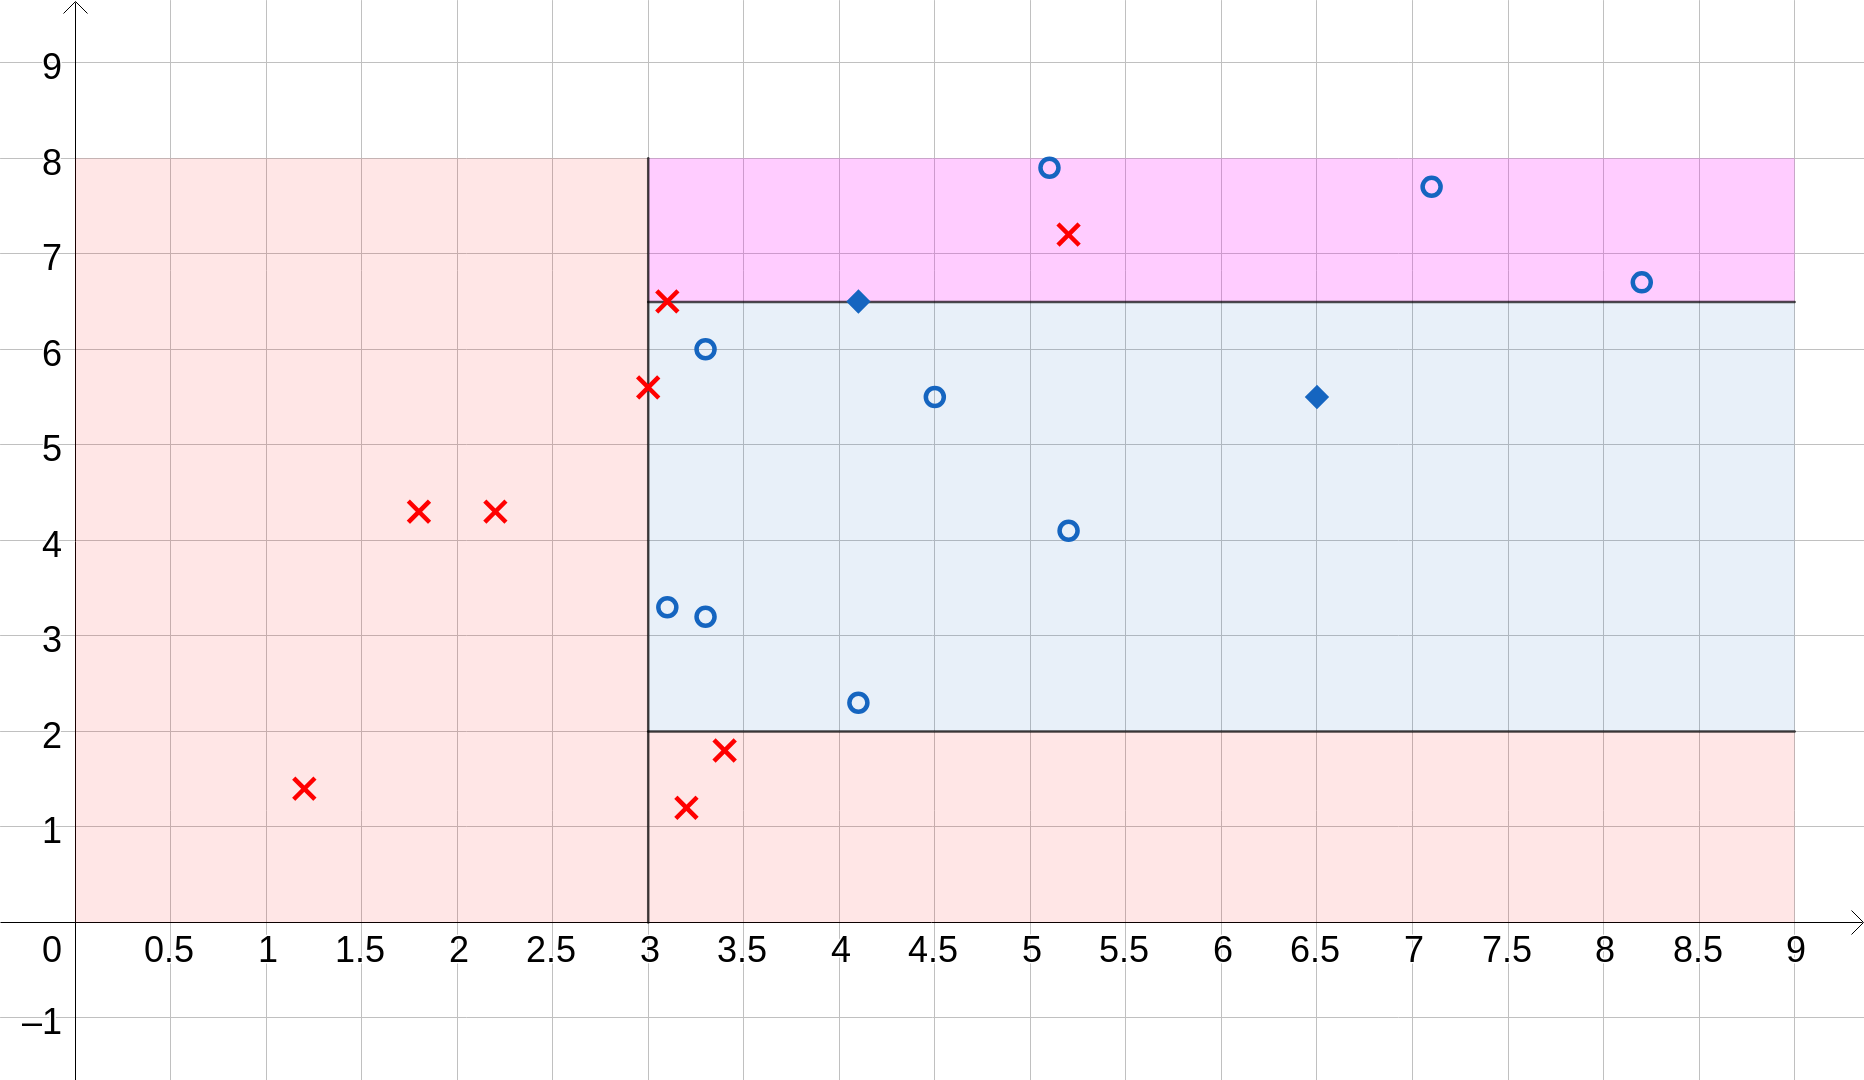
\includegraphics[width=.75\textwidth]{NewValues}
  \caption{Test values plotted into the graph split by regions}
  \label{NewValues}
\end{figure}

\end{document} 